% Section 1 - Introduction
% Alessandro Tenaglia <alessandro.tenaglia@uniroma2.it>
% May 6, 2022

% ### Introduction ###
\section{Introduction}
\graphicspath{{figs/section1/}}

% --- Overview ---
\begin{frame}{Overview}
	\begin{block}{Multi-threaded Application Real-Time executor}
		MARTe is a \textbf{C++ modular} and \textbf{multi-platform framework} for the development of \textbf{multi-threaded real-time control system applications}.
	\end{block}
\end{frame}

% --- MARTe1 ---
\begin{frame}{MARTe1}
	\begin{columns}
		\column{.5\textwidth}
		\begin{itemize}
			\item \textbg{MARTe1} is the previous version of this framework;
			\item \textbg{MARTe1} was deployed in many fusion real-time control systems, i.e. JET tokamak;
			\item The use of \textbg{MARTe1} increased the number of supported environments and platforms;
		\end{itemize}
		\column{.5\textwidth}
		\begin{figure}
			\centering
			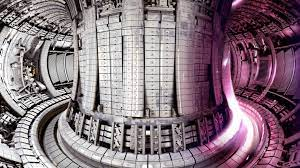
\includegraphics[scale=.5]{JET.jpeg}
			\label{fig:jet}
			\caption{JET Tokamak}
		\end{figure}
	\end{columns}
\end{frame}
